\todo{Esto estaba marcado}En este capítulo tratamos las distintas escalas de longitud dentro de la dinamica de los nucleones en condiciones acordes a las de la corteza de las estrellas de neutrones, estudiando materia simétrica en isospín (igual cantidad de protones y neutrones) a densidades menores a la de saturación para 5000 partículas.
Variando la temperatura encontramos una tranisición de fase sólido-líquido que se puede caracterizar también como una transición topológica.
Para temperaturas más altas que la de la transición de fase estudiamos la opacidad de los neutrinos y encontramos que en la fase líquida el \emph{scattering} de los neutrinos de bajo momento se mantiene elevado, incluso con morfologías que son significativamente diferentes a las de la pasta nuclear tradicional.


\section{Introducción}

En este capítulo utilizamos distintas herramientas topológicas y termodinámicas para caracterizar la materia de estrellas de neutrones simétrica.

\subsection{Herramientas Topológicas}

Una de las herramientas topológicas que utilizamos son los funcionales de Minkowski.
Las medidas topológicas de un cuerpo convexo $K \in \mathcal{R}$ se definen como funcionales $\varphi: \mathcal{R} \rightarrow \mathbb{R}$ que satisfacen tres propiedades:

\begin{description}
  \item{Invariancia de movimiento:} $\varphi(K) = \varphi(g(K))$, donde $g(K)$ implica cualquier tipo de traslación y rotación del cuerpo $K$.
  \item{Aditividad:} $\varphi(K_1 \cup K_2) = \varphi(K_1) + \varphi(K_2) - \varphi(K_1 \cap K_2)$.
  \item{Continuidad:} $\lim_{n\rightarrow\infty}\varphi(K_n) = \varphi(K)$ si $\lim_{n\rightarrow\infty}K_n = K$, donde ${K_n}$ es un conjunto de cuerpos convexos.
\end{description}

El teorema de Hadwiger dice que para un sistema de dimensión $d$ hay sólo $d+1$ funcionales independientes que satisfacen las propiedades mencionadas: las funcionales de Minkowski. En el espacio tridimensional, las funcionales de Minkowski están asociadas al volumen, el área, la curvatura media y el número de Euler. A pesar de que no necesariamente las estructuras obtenidas en este trabajo sean convexas (es decir, las funcionales de Minkowski no las definen unívocamente), utilizamos estas medidas para caracterizarlas. En el apéndice~\ref{ap:minkowski} se puede observar detalladamente el cálculo de estas magnitudes.

Además de las funcionales de Minkowski, utilizamos la función distribución de pares, usualmente denominada $g(r)$, que se define a partir de un histograma de todas las distancias entre pares de partículas.
Este histograma luego se normaliza con respecto al del gas ideal, donde las distancias están completamente descorrelacionadas.
Para tres dimensiones, esta normalización es la densidad multiplicada por el volumen de un cascarón esférico.

\subsection{Herramientas Termodinámicas}

Además de las clásicas señales termodinámicas para las transiciones de fase de primer o segundo orden, utilizamos el coeficiente de Lindemann.
El coeficiente de Lindemann se basa en la idea del desorden de las partículas, y es utilizado especialmente para estudiar transiciones de tipo sólido-líquido en sistemas infinitos, como los cristales.
Se define a partir de la desviación estándar de las posiciones de las partículas, $\Delta
r_i^2$:

\begin{equation*}
\Delta_L = \frac{\sqrt{\sum_i\langle\Delta r_i^2/N\rangle}}{a}
\end{equation*}
donde $a$ es la constante de red del cristal y $N$ el número total de partículas.
En nuestro caso, escogenos $a=(V/N)^{1/3}$, la longitud característica del sistema.


\section{Transición de fase}\label{phase_transition}
\subsection{Transición de fase termodinámica}

La figura~\ref{fig:energy} presenta la energía como función de la temperatura (curva calórica) para distintas densidades.
Cada una de estas densidades exhibe una discontinuidad en la energía para ciertas temperaturas, una señal de una transición de fase de primer orden.
Esta transición puede ser confirmada y caracterizada como de sólido-líquido observando el coeficiente de Lindemann. Por ejemplo, mostramos el coeficiente de Lindemann junto a la energía para $\rho=0.05\,\text{fm}^{-3}$ en la figura~\ref{fig:lind-energ}.
Esta figura muestra que las discontinuidades en las energía y en el coeficiente de Lindemann están a la misma temperatura.
Éstas dos son características de la transición de fase sólido-líquido.

\begin{figure}[h!]  \centering
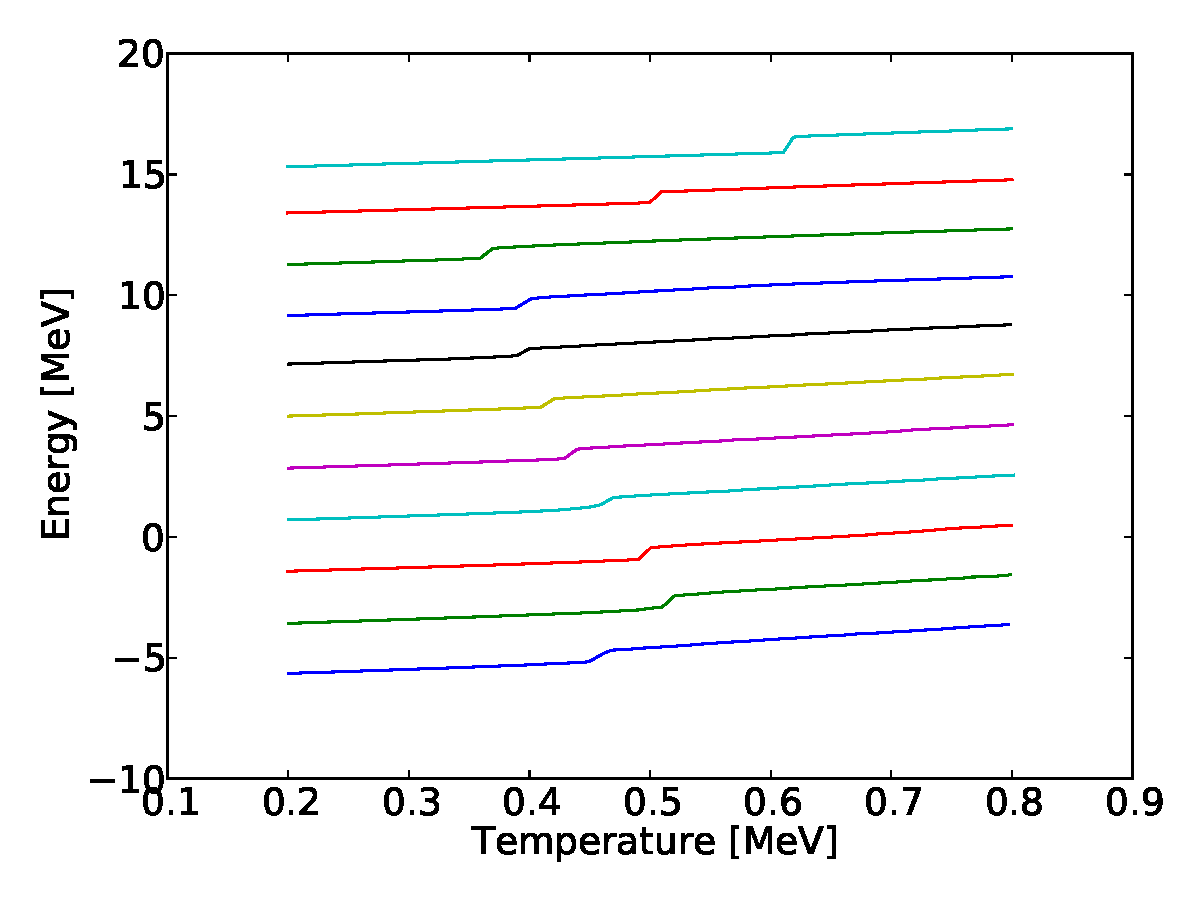
\includegraphics[width=0.4\columnwidth]{transicion/energy.pdf}
\caption{Energía como función de la temperatura para distintas densidades.
  Observamos una discontinuidad en el rango desde $T_l=0.35\,\text{MeV}$ a $T_h=0.65\,\text{MeV}$, dependiendo de la densidad.
  Esto es una señal de una transición de fase.
  En la figura, las densidades van de $\rho=0.03\,\text{fm}^{-3}$ a $\rho=0.13\,\text{fm}^{-3}$, incrementando $\Delta\rho=0.01\,\text{fm}^{-3}$ hacia arriba.}
\label{fig:energy}
\end{figure}

\begin{figure}[h!]  \centering
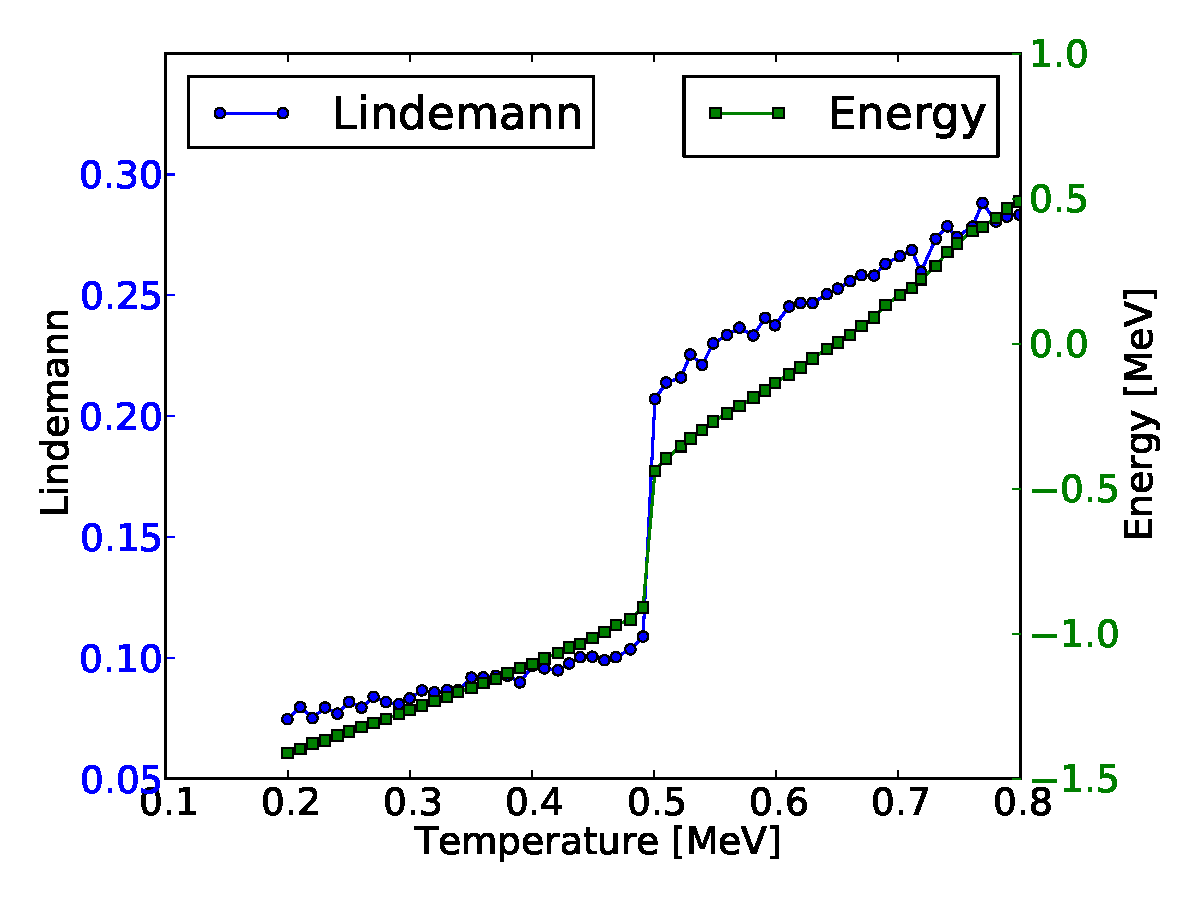
\includegraphics[width=0.4\columnwidth]{transicion/lind-energ.pdf}
\caption{Coeficiente de Lindemann y energía como función de la temperatura para una densidad, $\rho=0.05\,\text{fm}^{-3}$.
  El cambio abrupto en su valor es una señal de una transición de fase sólido-líquido.
  Podemos ver que ambas discontinuidades están a la misma temperatura.}
\label{fig:lind-energ}
\end{figure}

En la figura~\ref{fig:rdf} mostramos la función de distribución de pares para tres densidades distintas: $\rho=0.03\,\text{fm}^{-3}$ (\emph{spaghetti}), $\rho=0.05\,\text{fm}^{-3}$ (\emph{lasagna}) y $\rho=0.08\,\text{fm}^{-3}$ (túneles), inmediatamente sobre y bajo la temperatura de transición, así como una foto del sistema en la fase de temperatura alta.
Como los primeros picos (correspondientes a los primeros vecinos) están en la misma posición más allá de la temperatura, comcluimos que el orden corto está present tanto sobre como bajo la transición.
Sin embargo los los picos de los terceros vecinos, distintivos de las fases sólidas, desaparecen a medida que la temperatura aumenta más allá de la transición.
El orden de muy largo rango también sobrevive a la transición, como discutimos más adelante en la sección~\ref{very_long}

\begin{figure*}[floatfix]
  \centering
  \begin{subfigure}[h!]{0.4\columnwidth}
    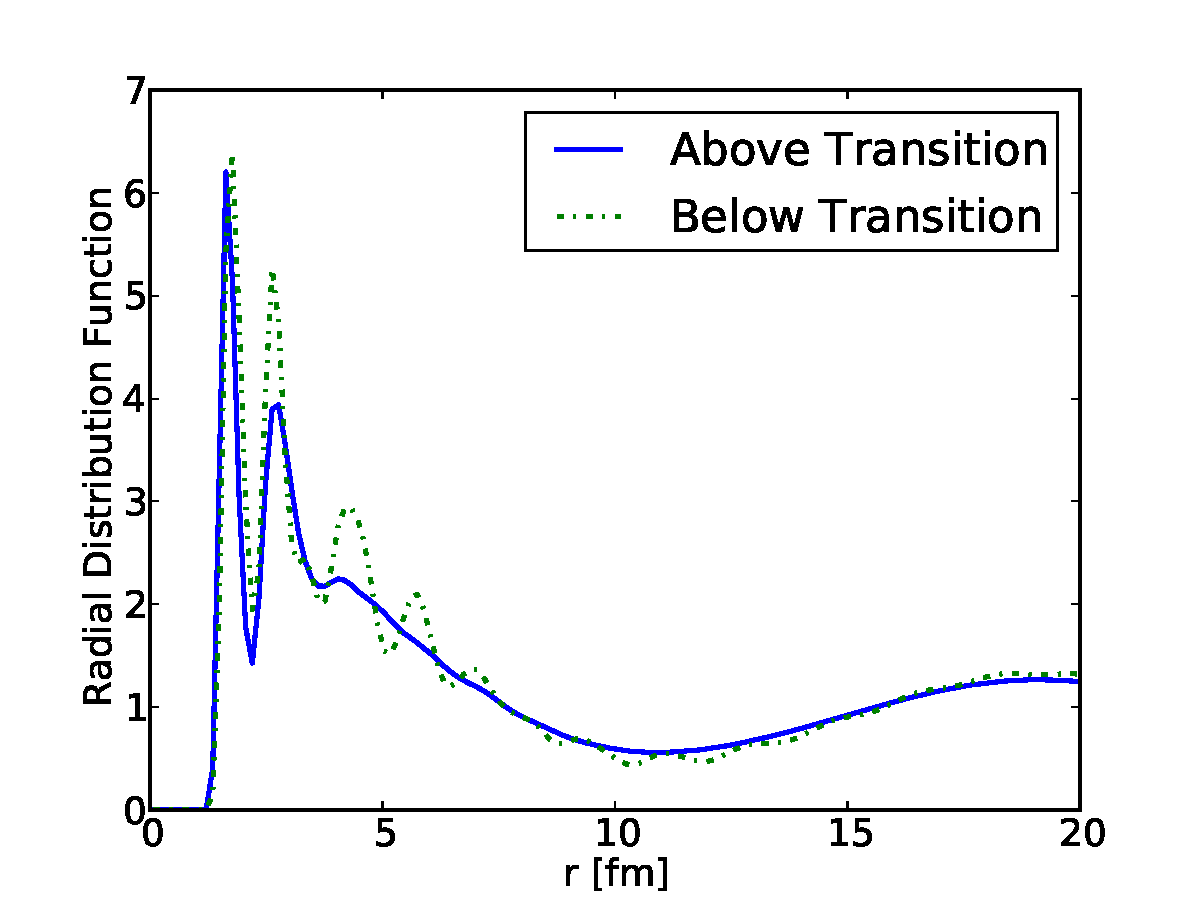
\includegraphics[width=\columnwidth]{transicion/rdf_0-03.pdf}
    \caption{Función de distribución de pares para $\rho=0.03\,\text{fm}^{-3}$}
  \end{subfigure}
  \begin{subfigure}[h!]{0.3\columnwidth}
    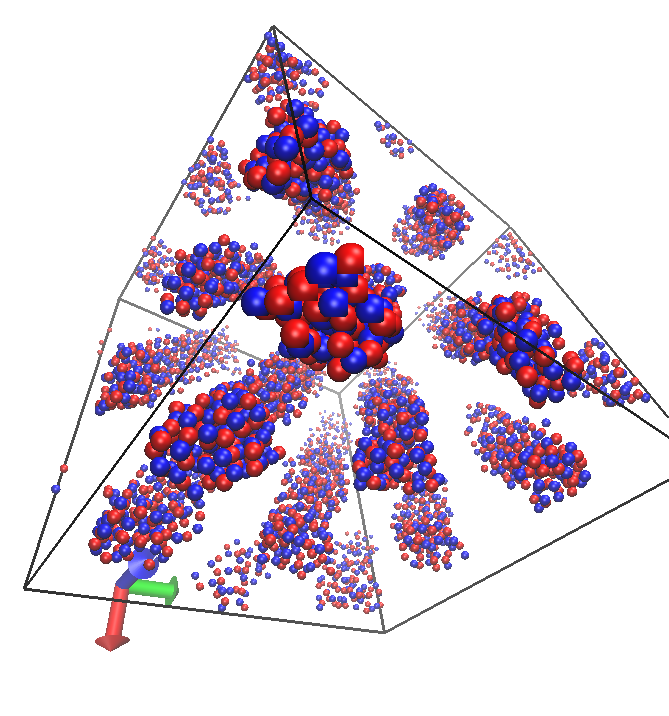
\includegraphics[width=\columnwidth]{transicion/morph_0-03_0-47.png}
    \caption{Foto del sistema en la fase líquida para $\rho=0.03\,\text{fm}^{-3}$}
  \end{subfigure}
  \begin{subfigure}[h!]{0.4\columnwidth}
    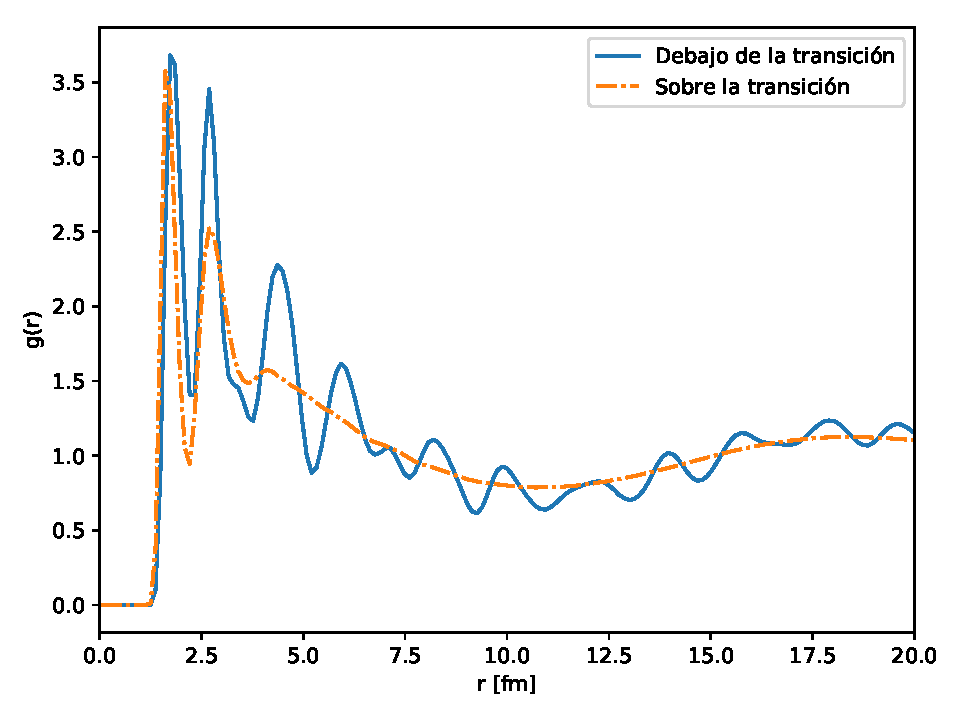
\includegraphics[width=\columnwidth]{transicion/rdf_0-05.pdf}
    \caption{Función de distribución de pares para $\rho=0.05\,\text{fm}^{-3}$}
  \end{subfigure}
  \begin{subfigure}[h!]{0.3\columnwidth}
    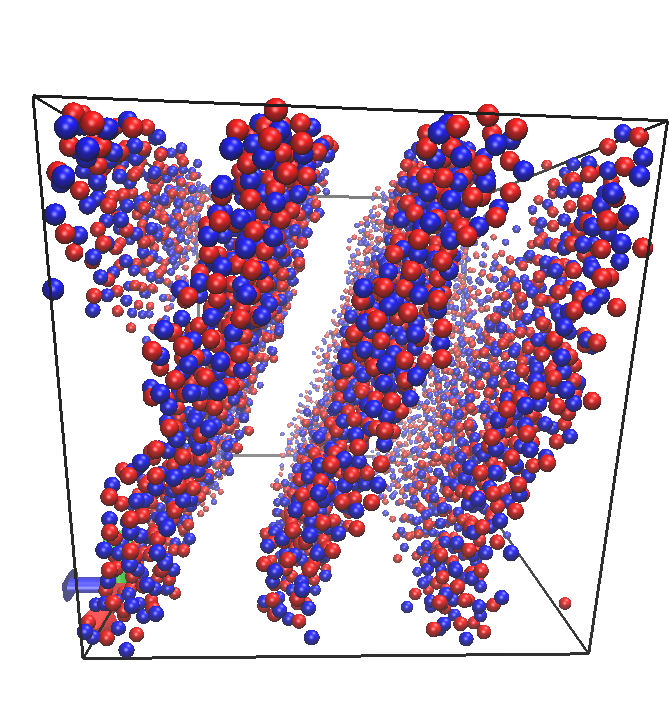
\includegraphics[width=\columnwidth]{transicion/morph_0-05_0-50.png}
    \caption{Foto del sistema en la fase líquida para $\rho=0.05\,\text{fm}^{-3}$}
  \end{subfigure}
  \begin{subfigure}[h!]{0.4\columnwidth}
    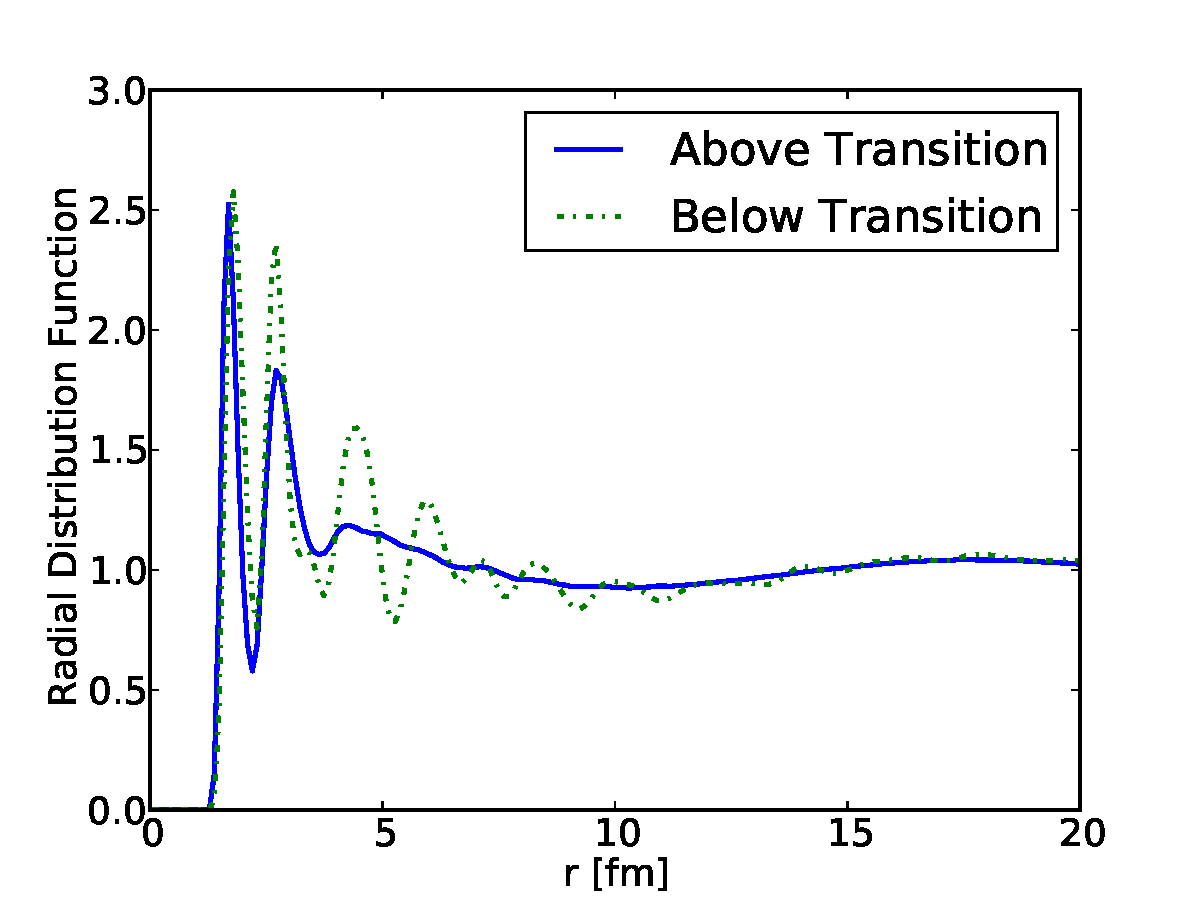
\includegraphics[width=\columnwidth]{transicion/rdf_0-08.pdf}
    \caption{Función de distribución de pares para $\rho=0.08\,\text{fm}^{-3}$}
  \end{subfigure}
  \begin{subfigure}[h!]{0.3\columnwidth}
    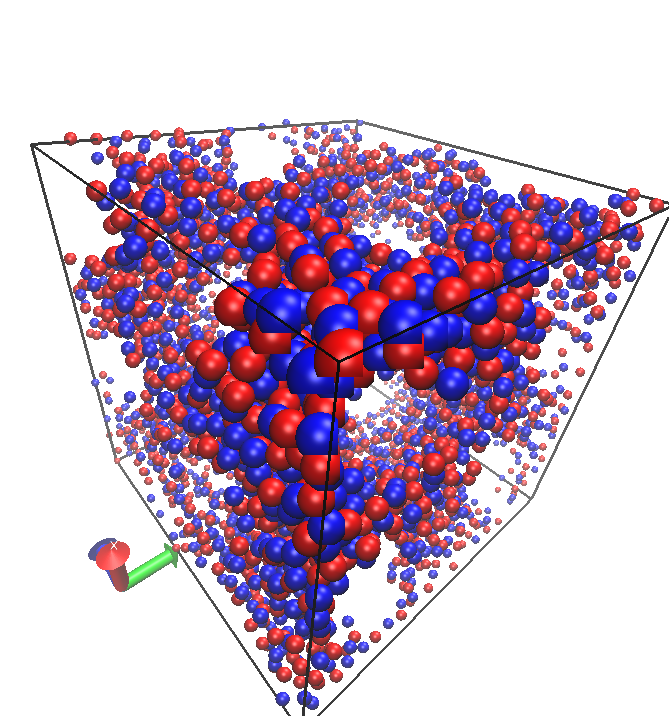
\includegraphics[width=\columnwidth]{transicion/morph_0-08_0-42.png}
    \caption{Foto del sistema en la fase líquida para $\rho=0.08\,\text{fm}^{-3}$}
  \end{subfigure}
  \caption{Función de distribución de pares para distintas densidades, tanto debajo como sobre la temperatura de transición, y foros del sistema en la fase líquida.
Aunque los pirmeros picos de la distribución están en las mismas posiciones para ambas temperaturas, los picos siguientes, que exhiben un orden de rango largo típico de los sólidos, sólo están presentes por debajo de la temperatura de transición.}
  \label{fig:rdf}
\end{figure*}

\subsection{Transición de fase topológica}
Cuando observamos los funcionales de Minkowski, particularmente la característica de Euler y el ancho medio, observamos que también hay una temperatura ``crítica'' en la cual ambas magnitudes exhiben una transición abrupta.
Mostramos, como un ejemplo, estas magnitudes como función de la temperatura para la densidad
$\rho=0.05\,\text{fm}^{-3}$ en la figura~\ref{fig:euler-curv}.
Como esta transición está señalada por los observables topológicos, concluimos que es una transición también topológica.
\todo[inline]{Explicar que es por los agujeros}

\begin{figure}%[H]
  \centering 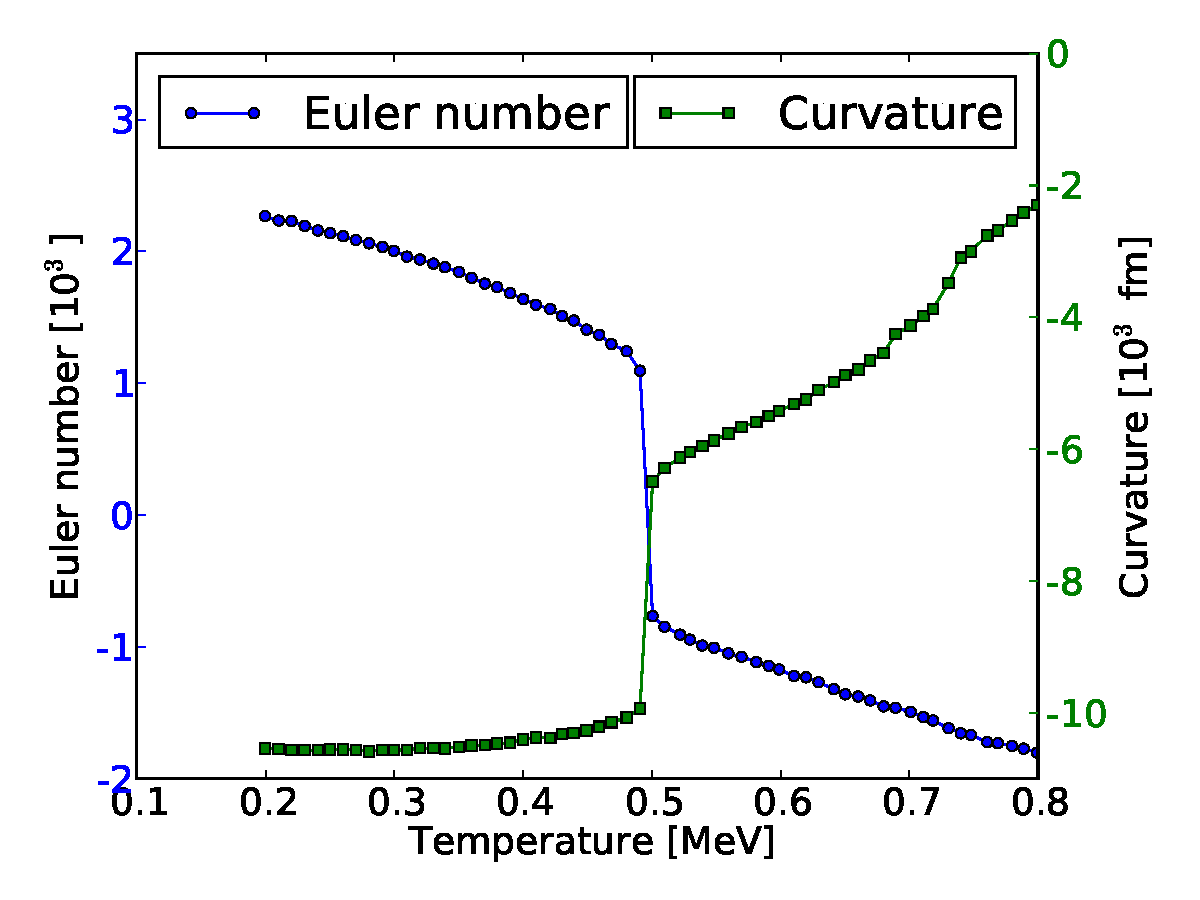
\includegraphics[width=0.4\columnwidth]{transicion/euler-curv.pdf}
  \caption{Número de Euler y ancho medio para $\rho=0.05\,\text{fm}^{-3}$.
    Observamos una transición abrupta para ambas funcionales de Minkowski.}
  \label{fig:euler-curv}
\end{figure}

Estas señales de una transición sólido-líquido (discontinuidad en la energía y en el coeficiente de Lindemann) y topológica (discontinuidad en las funcionales de Minkowski) se producen a la misma temperatura de transición, como se puede observar en el diagrama de fases de la figura~\ref{fig:critical_temperature}.
Esto significa que, a medida que el sistema es enfriado a un volumen fijo, sufre una transición termodinámica y topológica a la misma temperatura.
\todo{Acá pusiste que la topológica es cuando aparecen las inhomogeneidades. Es verdad, yo quiero decir que tiene otro cambio cuando se congelan esas inhomogeneidades. No sé cómo hacer que quede claro}

\begin{figure}[floatfix]  \centering
  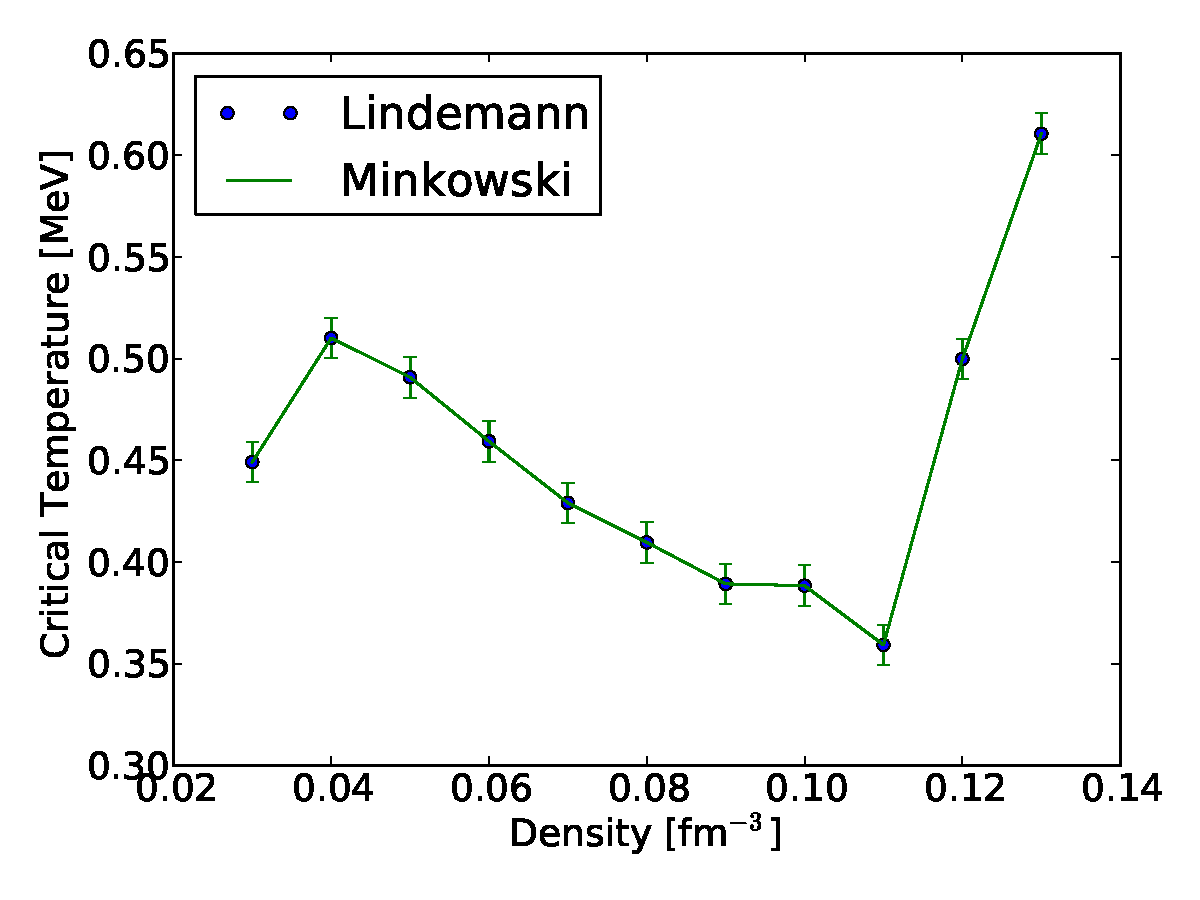
\includegraphics[width=0.4\columnwidth]{transicion/critical_temperature.pdf}
  \caption{Temperatura crítica como función de la densidad.
    Observamos la superposición entre la temperatura crítica de las funcionales de Minkowski y el coeficiente de Lindemann.}
  \label{fig:critical_temperature}
\end{figure}


\section{Comportamiento de muy largo rango}\label{very_long}
Además de que desaparece el orden de corto largo característico de los sólidos, otra característica es evidente de la figura~\ref{fig:rdf}.
Una modulación de muy largo en la función de distribución de pares sobrevive a través de la transición de sólido-líquido.
Este orden de muy largo rango es característico de las fases de la pasta.
En la figura~\ref{fig:morph} mostramos la configuración espacial para $\rho=0.05\,\text{fm}^{-3}$, para temperaturas tanto sobre como debajo de la temperatura de transicion.
En ella vemos que no sólo la fase sólida tiene la forma usual de la plasta, sino que además la fase líquida la preserva.
Debajo de a transición, tenemos ``pasta congelada''.
Justo por sobre ella, los nucleones pueden fluir, pero confinados a cierta pasta o estructura tipo-pasta, como vemos en las siguientes secciones.

\begin{figure*}[floatfix]%[H]
  \centering
  \begin{subfigure}[h!]{0.3\columnwidth}
    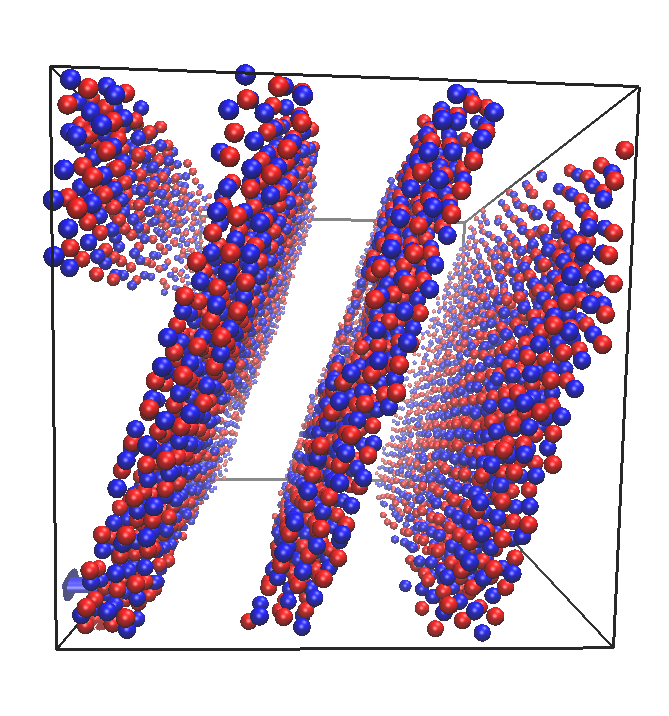
\includegraphics[width=\columnwidth]{transicion/morph_0-05_0-48.png}
    \caption*{Debajo de la transicion.}
  \end{subfigure}
  \begin{subfigure}[h!]{0.3\columnwidth}
    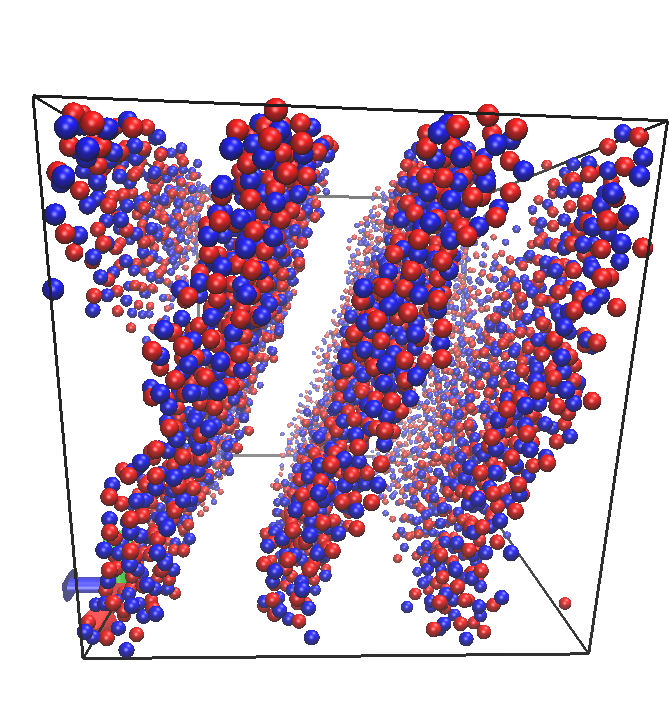
\includegraphics[width=\columnwidth]{transicion/morph_0-05_0-50.png}
    \caption*{Sobre la transición.}
  \end{subfigure}
  \caption{Distribución espacial para $\rho=0.05\,\text{fm}^{-3}$, tanto sobre como debajo de la temperatura de transición.
    Las estructuras son similares, pero mucho más desordenadas sobre la transición.}
  \label{fig:morph}
\end{figure*}

\section{Propiedades de transporte de neutrinos}
Este orden de muy largo rango, evidente de la figura~\ref{fig:rdf}, es responsable del pico a muy bajo momento $k$ ($\sim 10\,\text{fm}$ wave-length) en el factor de estructura $S(k)$, proporcional a la probabilidad de scattering.
Con esto en mente, ahora nos enfocamos en el orden de muy largo rango para nuestras estructuras.

En la figura~\ref{fig:sk_peak_0-05} graficamos la altura del pico del factor de estructura para momentos bajos $S(k<0.5\,\text{fm}^{-1})$ ($\lambda\gtrsim13\,\text{fm}$) como función de la temperatura para $\rho=0.05\,\text{fm}^{-3}$.
La forma más intuitiva para leer esta figura es de derecha a izquierda (de temperaturas altas a bajas), reproduciendo el procedimiento de enfriado del sistema en nuestras simulaciones.
Cada línea corresponde a evoluciones con distintas condiciones iniciales, pero manteniendo el mismo protocolo de enfriameiento y los mismos criterios de estabilidad.

\begin{figure}
  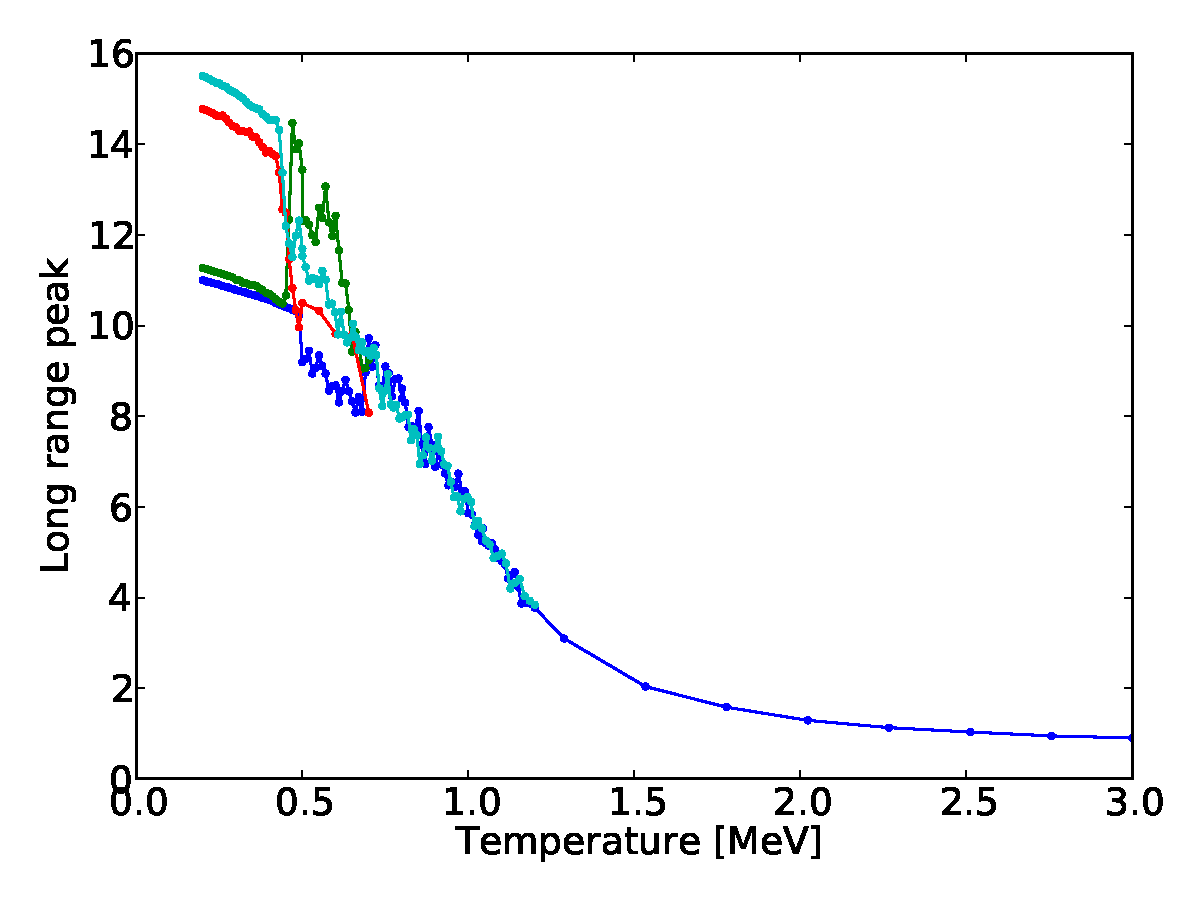
\includegraphics[width=0.4\columnwidth]{transicion/sk_peak_0-05.pdf}
  \caption{Pico de $S(k)$ para momentos bajos como función de la temperatura, para $\rho=0.05\,\text{fm}^{-3}$.
    Observamos dos comportamientos para $T<0.5\,\text{MeV}$ y $T>0.5\,\text{MeV}$.  }
  \label{fig:sk_peak_0-05}
\end{figure}

A temperaturas altas los nucleones están distribuidos de forma bastante homogénea, y no se evidencia ninguna estructura a partir de la $S(k)$: el ``pico'' desaparece, tendiendo a 1 (el valor para sistemas homogéneos).
A medida que la temperatura decrece aparece un pico en los momentos bajos.
La transición descripta en la sección \ref{phase_transition} se manifiesta en la figura~\ref{fig:sk_peak_0-05} a partir de la ausencia de fluctuaciones para temperaturas menores a la de transición $T \lesssim 0.5\,\text{MeV}$.
Incluso a temperaturas altas como
$T=1.0\,\text{MeV}$ aún hay un pico de absorción reconocible para momentos bajos (con altura claramente mayor a 1), pero no siempre se corresponde a la forma de una pasta usual (\emph{gnocchi}, \emph{spaghetti} o
\emph{lasagna}) en nuestras simulaciones.
A estas temperaturas, y para la mayoría de las densidades, la estructura del sistema es parecida a una ``esponja'' que es, de cualquier modo, suficientemente ordenada como para producir un pico reconocible en $S(k)$.

Es interesante notar que cuando el sistema llega a temperaturas de $T\sim 0.7\,\text{MeV}$ observamos que distintas ejecuciones de la simulación causan que el sistema ``colapse'' en distintas estructuras, además de la \emph{lasagna} usual.
Podemos observar en detalle la altura del pico de  $S(k)$ para esta región de temperaturas en la figura~\ref{fig:sk_peak_zoom} y las estructuras que corresponden a cada una de las simulaciones en la figura~\ref{fig:cool_morph} (ver epígrafe para detalles).

\begin{figure}
  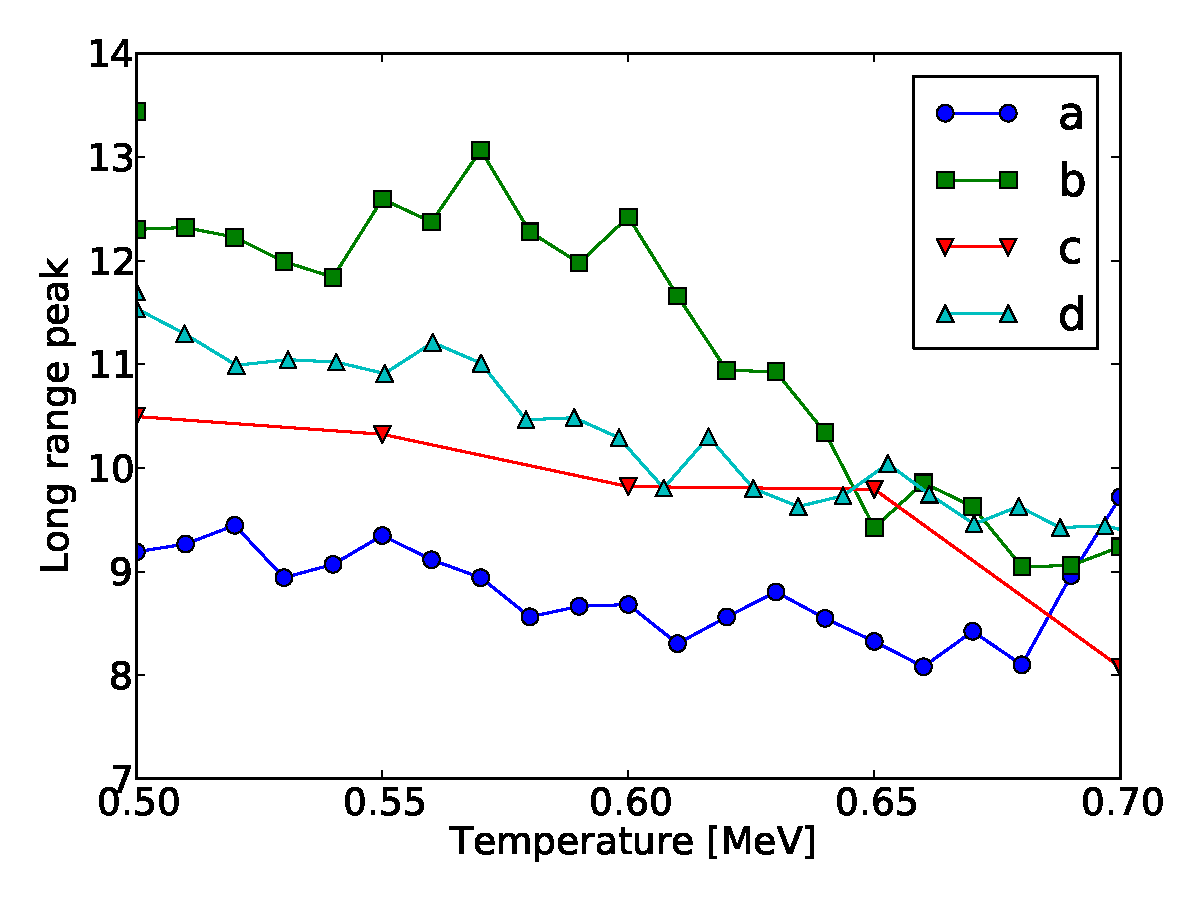
\includegraphics[width=0.4\columnwidth]{transicion/sk_peak_zoom.pdf}
  \caption{Pico de $S(k)$ para momentos bajos, en el rango de temperaturas entre $T=0.5\,\text{MeV}$ and $T=0.7\,\text{MeV}$.
    Observamos que distintas condiciones iniciales conducen a distintos picos de abosrción para bajos momentos.}
  \label{fig:sk_peak_zoom}
\end{figure}


\begin{figure*}[floatfix]%[H]
  \centering
  \begin{subfigure}[h!]{0.3\columnwidth}
    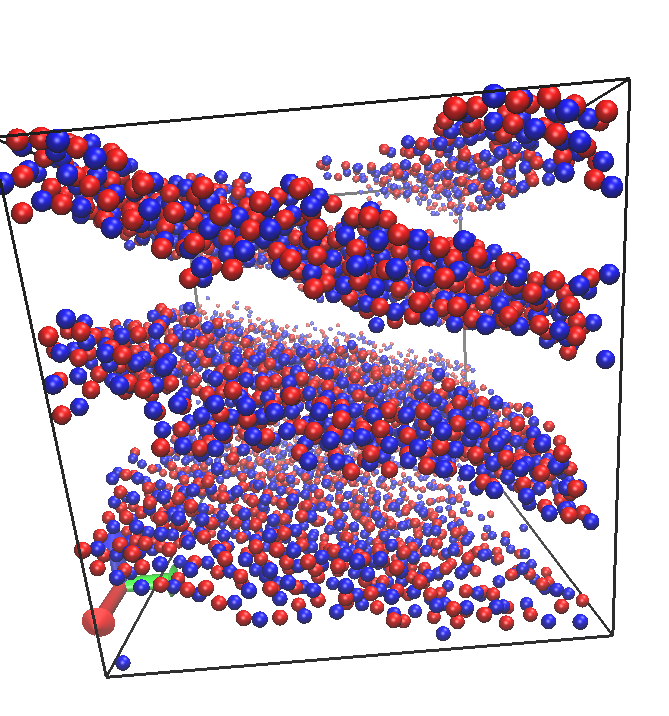
\includegraphics[width=\columnwidth]{transicion/morph_02-08-001.png}
    \caption{\emph{Lasagna} usual}
  \end{subfigure}
  \begin{subfigure}[h!]{0.3\columnwidth}
    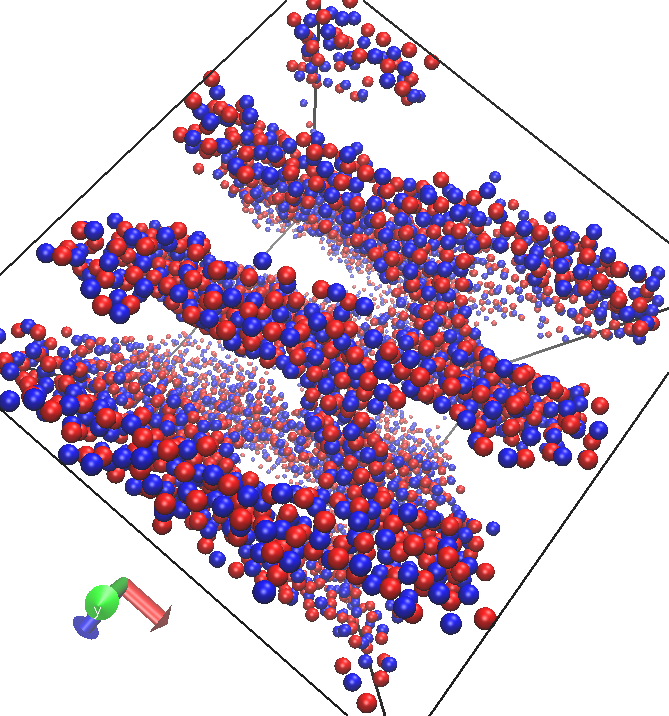
\includegraphics[width=\columnwidth]{transicion/morph_05-07-001.png}
    \caption{\emph{Lasagna} interconectada}
  \end{subfigure}
  \begin{subfigure}[h!]{0.3\columnwidth}
    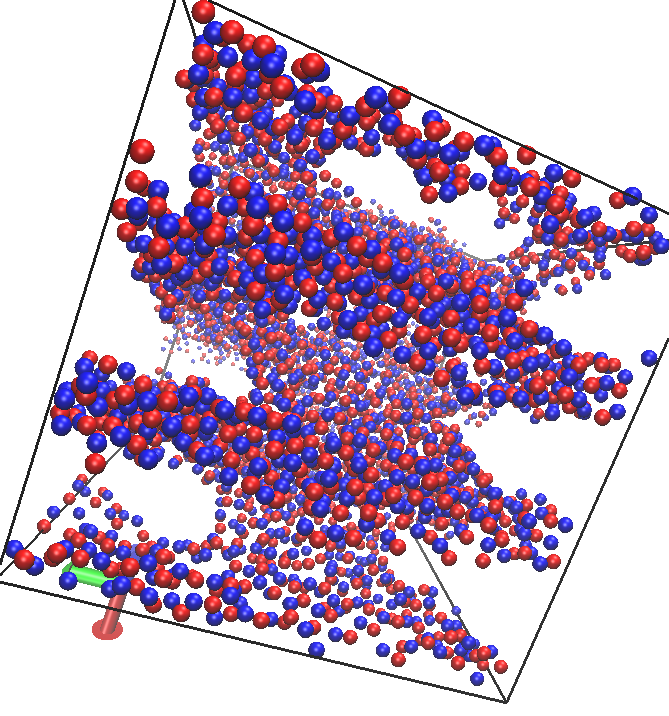
\includegraphics[width=\columnwidth]{transicion/morph_05-12-0013.png}
    \caption{\emph{Lasagna} interconectada}
  \end{subfigure}
  \begin{subfigure}[h!]{0.3\columnwidth}
    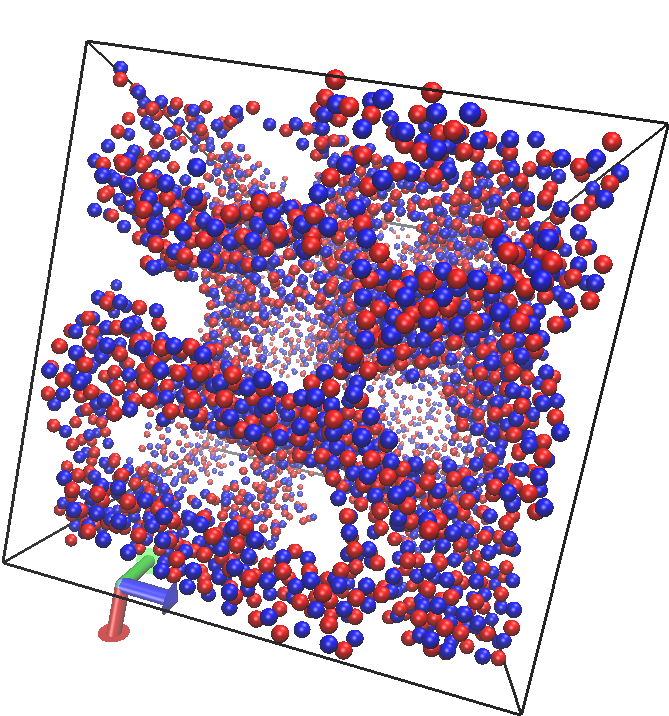
\includegraphics[width=\columnwidth]{transicion/morph_decorr.png}
    \caption{Pasta inusual}
  \end{subfigure}
  \caption{Estructuras del sistema para $\rho=0.05\,\text{fm}^{-3}$ para distintas condiciones iniciales.
    Podemos observar la \emph{lasagna} usual, pero también \emph{lasagnas} interconectadas y otras esctructuras que no se parecen a la pasta usual.
    A pesar de ser distintas de las formas de la pasta usual, estas estructuras tienen un pico para momentos bajos en el factor de estructura.}
  \label{fig:cool_morph}
\end{figure*}

\section{Propiedades de pasta no tradicional}
\label{unusual_pasta}

\todo[inline]{Las pastas usuales son estados de mínima energía potencial.
Estas estructuras no tradicinoales descriptas en la sección anterior son, probablemente, mínimos \emph{locales} de energía potencial, que abundan en sistemas frustrados como éste.
La complejidad del \todo[inline]{paisaje de la energía} (muchos mínimos locales separados por barreras de energía) hacen difícil alcanzar el estado de mínima energía simplemente enfriando en simulaciones de dinámica molecular.
Sin embargo, como estamos trabajando con un número fijo de partículas, volumen y temperatura (ensambe $(N,V,T)$
), el estado de equilibrio a temepraturas finitas no es el que minimiza la energía interna, sino e que minimiza la energía libre de Helmholtz, $A = E - T\,S$.
Todas estas estructuras, en conclusión \emph{podrían ser} la solución de equilibrio.
}
Cálculos precisos de energías libres a partir de simulaciones de dinámica molecular son muy costosos computacionalmente~\cite[pp. 167-200]{frenkel_understanding_2001}, especialmente a bajas temperaturas, cuando sobrepasar las barreras de energía es un evento muy poco probable.
Sin embargo, podemos calcular fácilmente las distribuciones de energía interna en una evolución temporal a temperatura constante.
En la figura~\ref{fig:histo} mostramos los histogramas de energía construidos a partir de sistemas termalizados en una muy larga evolución, a temperatura $T=0.6\,\text{MeV}$, utilizando tres de los sistemas mostrados en~\ref{fig:cool_morph} como condiciones iniciales.
Podemos ver que, a pesar de que los histogramas difieren claramente, se superponen bastante.
Esto indica que el ensamble de configuraciones de equilibrio a $T=0.6\,\text{MeV}$ puede contener cualquiera de estas estructuras, no sólo \emph{lasagna}.
A la luz de esto, proponemos que a temperaturas bajas pero finitas, el estado del sistema debería ser descripto como un ensamble de pastas tradicionales y no tradicionales.

Cuando calentamos el sistema hasta $T=0.8\,\text{MeV}$ estos tres histogramas se vuelve indistinguibles, dando a suponer que, para esta temperatura, se pueden superar las barreras de energía libre y el sistema es más probable que sea ergódico.

\begin{figure}[floatfix]%[H]
  \centering
  \begin{subfigure}[h!]{0.4\columnwidth}
    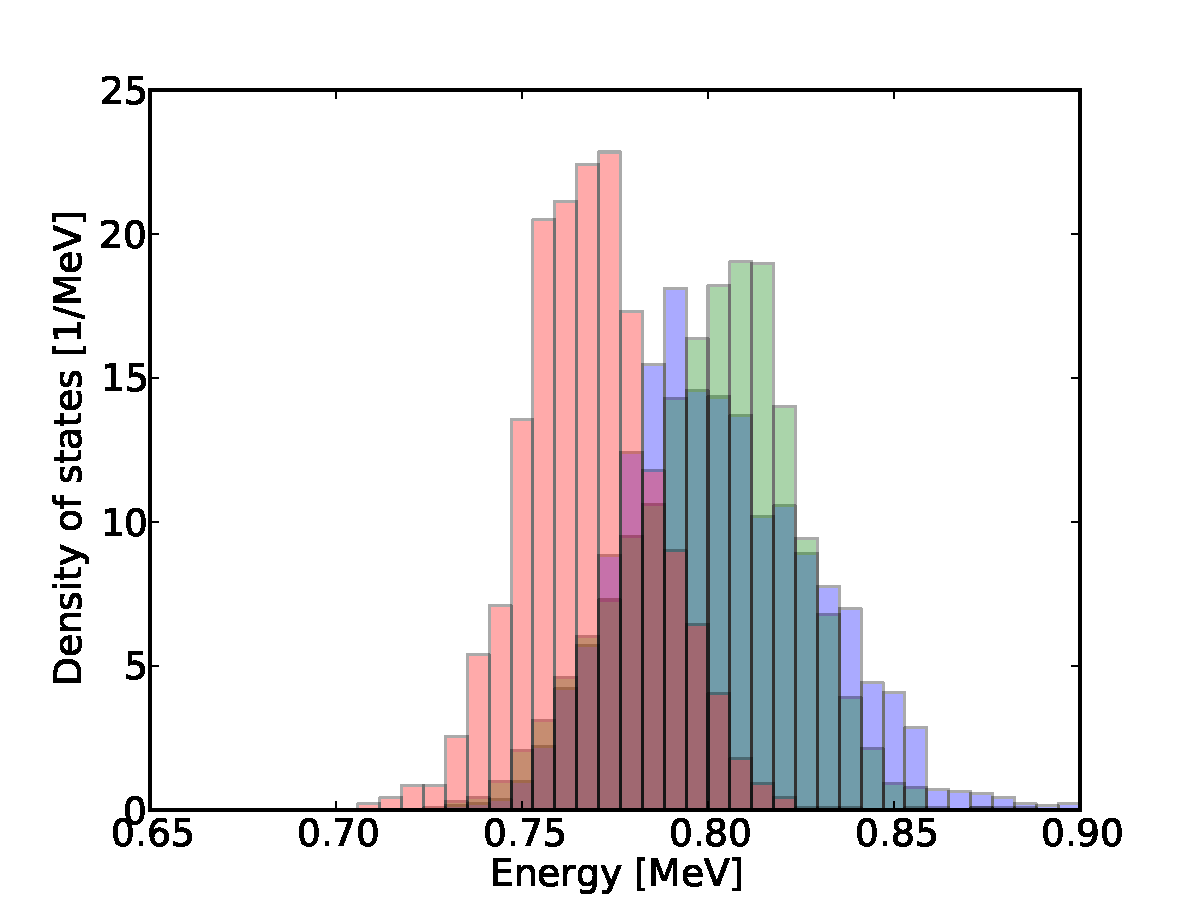
\includegraphics[width=\columnwidth]{transicion/histo_T_0-06.pdf}
    \caption{Distribución de energías para $T=0.6\,\text{MeV}$}
\label{subfig:histo_T_0-06}
  \end{subfigure}
  \begin{subfigure}[h!]{0.4\columnwidth}
    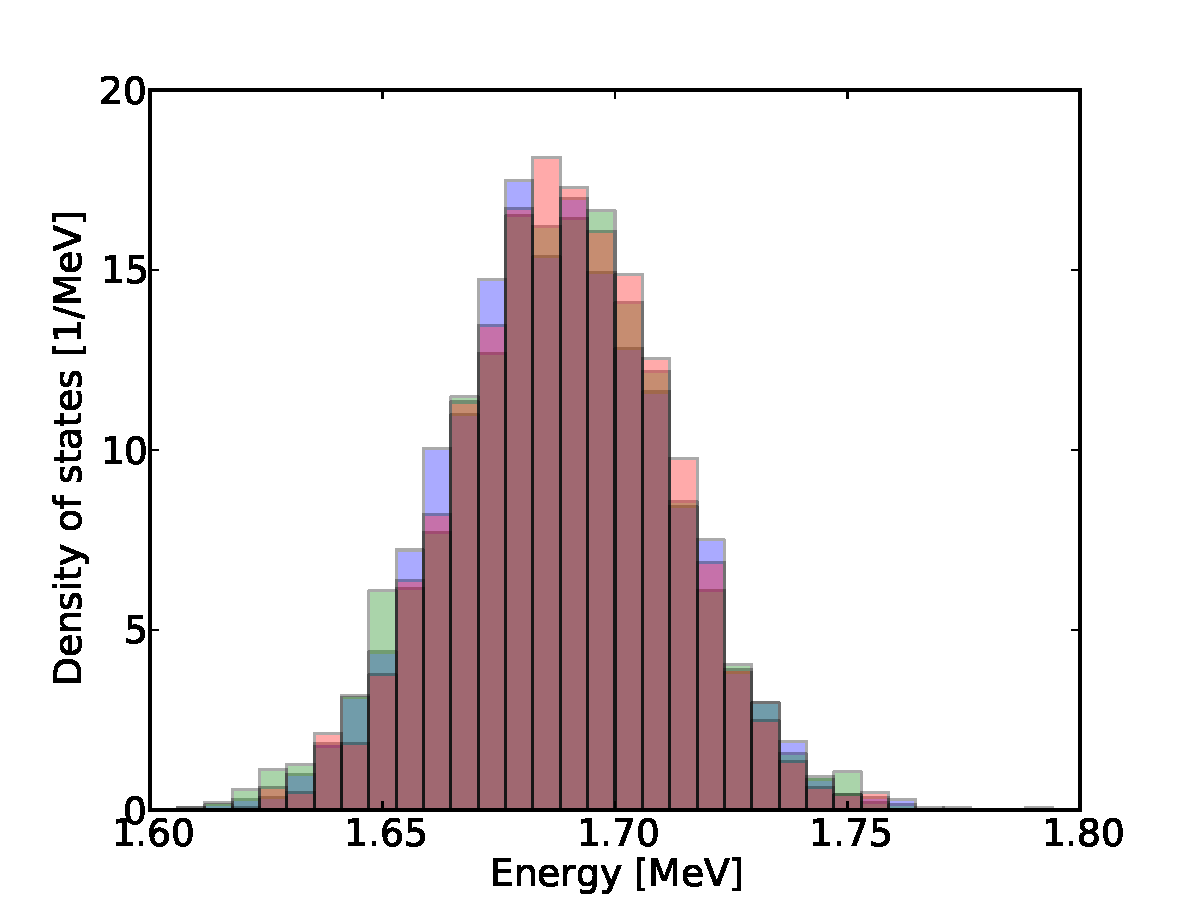
\includegraphics[width=\columnwidth]{transicion/histo_T_0-08.pdf}
    \caption{Distribución de energías para $T=0.8\,\text{MeV}$}
\label{subfig:histo_T_0-08}
  \end{subfigure}
  \caption{Distribución de energías para un esamble canónico.
    Se puede observar que, para $T=0.8\,\text{MeV}$, las tres distribuciones se solapan completamente.
    Sin embargo, para $T=0.6\,\text{MeV}$, los histogramas, aunque aún se solapan significativamente, están separados.}
\label{fig:histo}
\end{figure}

Estas observaciones son relevantes porque todas estas estructuras muestran picos en $S(k)$ a la misma longitud de onda, aunque alturas distintas.
Y, más importante, encontramos que estas estructuras que parecen sin forma pueden ser incluso más eficientes en el \emph{scattering} de neutrinos que cualquier pasta usual, a pesar de que éstas son usualmente invocadas como una necesidad para el \emph{scattering} coherente de neutrinos.
Este resultado muestra que pastas inusuales también deben ser consideradas cuando estudiamos la estructura de la corteza de las estrellas de neutrones.

\section{Conclusiones}
\label{discussion}

Encontramos una transición de fase de tipo sólido-líquido para todas las densidades estudiadas a temperaturas muy bajas.
Caracterizamos esta transición a través del coeficiente de Lindemann y de una discontinuidad en las curvas calóricas.
La transición también está marcada por una discontinuidad en los funcionales de Minkowski, y estos tres indicadores concuerdan en la misma temperatura de transición.
Esta transición no altera la forma típica de la pasta (\emph{lasagna} y \emph{spaghetti}
en los ejemplos mencionados): la fase líquida preserva la forma de la pasta encontrada en la fase sólida.

A medida que aumentamos la temperatura más allá de $T=0.7\,\text{MeV}$, las formas típicas de la pasta se vuelven inestables y el sistema adopta estructuras ligeramente más desodenadas, peor aún heterogéneas.
Sin embargo, el pico de absorción de bajo momento en estas estructuras se mantiene bastante elevado.
Esto implica que la existencia de formas tradicionales de pasta --que sólo se obtienen a temperaturas muy bajas-- no es una condición necesaria para la absorción de neutrinos en la corteza de las estrellas de neutrones.

Más aún, encontramos que a $T\sim0.7,\text{MeV}$ el sistema puede existir en varios estados estables, todos con distinta morfología --y, en consecuencia, distinto factor de estructura--, pero con energías internas muy cercanas.
A partir de nuestras simulaciones a $(N,V,T)$ fijos, estos estados parecen estar separados por barreras de energía relativamente altas, que hacen que la transición entre ellos sea un evento poco probable, no observado a partir de una sola simulación.
De todos modos, las distribuciones de energía obtenidas a partir de distintas condiciones inciales se solapan considerablemente, indicando que cualquiera de ellos puede ser el estado de equilibrio a esa temperatura.
A $T\sim0.8\,\text{MeV}$ las barreras de energías pueden ser superadas y los histogramas se solapan completamente.

Todo esto indica que el estado real de estos sistemas a temperatuars bajas, pero finitas, debe ser descripto a través del estudio de un ensamble de estructuras en vez de una sola estructura tipo pasta.